\documentclass[11pt,a4paper]{article}
\usepackage{fontspec}
\setmainfont{TeX Gyre Pagella}
\newfontfamily\headfont{Inter}[UprightFont=*-ExtraBold,BoldFont=*-ExtraBold,Extension=.otf,Path=/usr/share/fonts/opentype/inter/]
\usepackage[a4paper,margin=2.3cm]{geometry}
\usepackage{amsmath}
\usepackage{graphicx,booktabs,float,caption,array,xcolor,longtable,threeparttable}
\usepackage{xurl}
\usepackage[hidelinks]{hyperref}
\usepackage{titlesec}
\usepackage[round]{natbib}
\usepackage{setspace}
\setstretch{1.05}
\renewcommand{\topfraction}{0.9}
\renewcommand{\bottomfraction}{0.8}
\renewcommand{\textfraction}{0.1}
\renewcommand{\floatpagefraction}{0.75}
\setlength{\parindent}{0pt}
\setlength{\parskip}{0.55em}
\titleformat{\section}{\headfont\Large}{\thesection}{0.8em}{}
\titleformat{\subsection}{\headfont\large}{\thesubsection}{0.8em}{}
\captionsetup{font=small,labelfont=bf}
\urlstyle{same}
\hypersetup{pdftitle={Where the Lifeboats Go},pdfauthor={Dr Tristan Hotham}}

\begin{document}
\begin{center}
{\Large\bfseries Where the Lifeboats Go: Distance, Timing and Station Workload in 45,673 RNLI Lifeboat Launches, 2021 to 2025\par}
\vspace{1.2em}
{\large Dr Tristan Hotham\par}
\vspace{0.3em}
{\small Independent researcher\\
ORCID: 0000-0003-4931-9349\\
DOI: https://doi.org/10.5281/zenodo.24104520\par}
\vspace{0.8em}
2026
\end{center}

\begin{quote}
\small
\begin{center}\textbf{Abstract}\end{center}
Lifeboat services publish detailed records of their work, but these records are rarely analysed as a whole. I use the Royal National Lifeboat Institution's open Returns of Service, 45,673 lifeboat launches from 238 stations in the United Kingdom, Ireland, the Isle of Man and the Channel Islands in 2021 to 2025, to describe where lifeboats go, how far, for whom and when, following an analysis plan written before any outcome was computed. Half of all located launches went less than 4.5 km from the station in a straight line. Within the same station, all-weather lifeboats reached incidents 150\% further than inshore lifeboats (95\% CI 119 to 185), and commercial casualties lay 27\% further away than people in the water (CI 16 to 40); powered and sailing leisure craft did not differ detectably from people in the water. Demand from leisure craft was strongly seasonal: launches to powered and sail craft were 10.6 times as frequent in summer as in winter, against 2.2 times for commercial casualties, and leisure launches rose more at weekends. A station's workload was almost unrelated to the length of coast it is nearest to (elasticity 0.10, CI $-$0.02 to 0.22). Total launches were flat over the five years, but the share recorded with the casualty type ``Other'' rose from 8\% to 21\%, so declines in specific casualty groups cannot be separated from changes in recording. The analysis is descriptive and observational.

\textbf{Keywords:} maritime search and rescue; lifeboats; RNLI; coastal safety; spatial analysis; seasonality; open data
\end{quote}

\section{Introduction}
Every year the volunteer crews of the Royal National Lifeboat Institution (RNLI) launch their boats several thousand times. In the five years studied here they launched 45,673 times, about 25 times a day. Each launch is logged after the crew returns, in a record the RNLI calls a Return of Service: the station, the boat, the date and time, the kind of casualty, the reason for launching, the outcome, the weather and sea at the scene, and the position of the incident \citep{wright2021}. Since 2018 the RNLI has published these records, with the locations of its lifeboat stations, through an open data portal built with Esri \citep{roberts2018,rnlidata}. They are a detailed open record of maritime emergencies, yet, as far as I can tell, they have rarely been analysed as a whole outside the organisation itself.

This paper uses them to answer five plain questions. Where do lifeboats go, and how concentrated are those places? How far from the station do they go, and how does that differ between the two main kinds of lifeboat and between kinds of casualty? When do launches happen, across the year, the week and the day, and does the timing differ between leisure users of the sea and people who work on it? Which stations are busiest relative to the coast around them? And did the number and mix of launches change over the five years covered?

Each question has a practical side. The RNLI itself says it uses predictive modelling to judge whether its boats and stations are in the right places \citep{wright2021}, and a body of operational research addresses the placement of rescue boats \citep{razi2016,akbari2018}. What the open records allow is something different and complementary: an outside, reproducible description of the demand that actually reached the lifeboats, against which assumptions about distance, timing and coverage can be checked. The questions also matter for coastal safety. If most demand comes from leisure use of the sea, concentrated in summer afternoons and at weekends, close to the shore and close to population, then prevention aimed at leisure users is likely to matter as much as rescue capacity.

The contribution is threefold. First, I document the data and their problems: a small share of incident positions with a lost minus sign on the longitude, a few impossible positions, training launches, a station missing from the station list, and, most importantly for any analysis of trends, a steady rise in the share of launches recorded with the casualty type ``Other''. Second, I report a set of descriptive estimates with uncertainty, under a written plan that fixed the hypotheses, models and checks before any outcome was computed, and I report the planned results whether or not they matched expectations. Third, I release aggregate data, code and an interactive map, so that others can extend the analysis.

The answers, in brief, are these. Half of all located launches went less than 4.5 km from the station, and 77\% less than 10 km. All-weather lifeboats went 2.6 times as far as inshore lifeboats at the median, and 150\% further when compared within the same station. Commercial casualties were further out than people in the water, but motorboats and yachts, against my expectation, were not. Launches to motorboats and yachts rose roughly tenfold from winter to summer, while launches to commercial casualties roughly doubled; leisure launches were also more frequent at weekends. Station workloads bore almost no relation to coast length: the busiest coastal stations per kilometre of coast were on the crowded coasts of Lancashire, Kent, Sussex, Devon and Dorset, and the single busiest station of all, Tower, sits on the River Thames in central London. Total launches were flat over the five years.

Section~\ref{sec:lit} sets out the background. Section~\ref{sec:data} describes the data and their cleaning, Section~\ref{sec:design} the plan and methods, Section~\ref{sec:results} the results and Section~\ref{sec:robust} the checks. Section~\ref{sec:disc} discusses limitations and Section~\ref{sec:conc} concludes.

\section{Background}\label{sec:lit}
\subsection{The RNLI and its lifeboats}
The RNLI was founded in 1824 and is a charity that operates the main lifeboat service around the coasts of the United Kingdom and Ireland, with stations also on the Isle of Man and the Channel Islands. An RNLI data product manager describes a fleet operating from 238 lifeboat stations, with more than 5,500 operational volunteer crew and a lifeguard service on about 253 beaches, and notes four stations on the River Thames \citep{wright2021}. The station list used here also has 238 stations.

Two main classes of boat matter for this paper. All-weather lifeboats (ALBs) are large, fast, self-righting boats designed to operate in any sea state; in 2021 to 2025 the Severn, Shannon, Tamar, Trent and Mersey classes appear in the records. Inshore lifeboats (ILBs) are smaller rigid-inflatable or inflatable boats (Atlantic 85, D class, E class on the Thames) suited to shallow water, surf, rocks and rivers. Many stations operate both. The RNLI also runs a few hovercraft and, in some places, rescue water craft. These differences in capability make a difference in where the boats can go, and are the basis of the first hypothesis below.

The RNLI is one of several organisations that respond to emergencies at sea and on the coast. A case study of open marine data by the Open Data Institute notes that the RNLI responds to about half of incidents, with police, fire and rescue and ambulance services among the others, and that RNLI lifeguards handled 17,356 incidents in 2019 while lifeboat crews launched 8,941 times \citep{odi2021}. The launches studied here are therefore a large but partial record of coastal emergencies: they show the demand that reached the lifeboats, not all demand.

\subsection{Search and rescue, drowning and coastal hazards}
Research on maritime search and rescue has mostly taken an operational view. Location models place rescue boats so as to shorten response times, cut costs or widen coverage of expected incidents, using past incidents as their input \citep{razi2016,akbari2018}; drift models forecast where a person or craft in the water will be found \citep{breivik2008}; and reliability studies have examined how the coordination of rescues by the UK coastguard performs \citep{norrington2008}. Closest to this paper, \citet{pitman2019} used six years of RNLI rescue records to relate lifejacket wear, environmental conditions, activity and time to rescue to fatality rates: lifejacket wear was associated with lower fatality rates, life-at-risk incidents and fatalities were higher than expected in winter, and survival fell as time to rescue lengthened. These studies treat the spatial and temporal pattern of demand as an input; this paper describes it.

A second literature concerns drowning and coastal hazards. Unintentional drowning accounts for an estimated 0.7\% of all deaths worldwide, more than 500,000 a year \citep{szpilman2012}. In the UK, fatal drownings are recorded in the Water Incident Database (WAID); an evaluation of its 2012 to 2019 records judged it a rigorous and transparent source while recommending further fields \citep{hills2021}, and a case-crossover analysis of the same records found that the risk of unintentional drowning rose by about 7\% for each 1 degree rise in daily maximum air temperature, an association seen in males only \citep{hills2024}. On beaches, rip currents cause a large share of rescues: about 71\% of the incidents in RNLI beach rescue records for Devon and Cornwall \citep{scott2007}. UK rip current incidents and their victims have been analysed by \citet{woodward2013}, and the types and hazard of rip currents are reviewed by \citet{castelle2016}; in Australia they cause more confirmed deaths a year than bushfires, floods and cyclones combined \citep{brander2013}. Rivers are a further, often overlooked setting for drowning \citep{peden2016}, which matters here because several RNLI stations work on rivers and lakes. Among boating-related drownings in Australia, alcohol was involved in about a quarter and most of those who drowned were not wearing a lifejacket \citep{willcoxpidgeon2019}. These literatures concern deaths and lifeguard rescues. The lifeboat records add the larger set of calls, fatal or not, that reached a lifeboat, and they make it possible to describe where and when that demand arises.

\subsection{The open data}
The RNLI's move to publish data was framed as an experiment with being ``open by default'' in order to lower barriers for organisations working on drowning prevention \citep{roberts2018}. The data are offered through an ArcGIS Hub portal in several formats, alongside lifeguard units, survey results and annual statistics \citep{rnliresearch}. They are published under a bespoke licence, adapted from the Open Government Licence, which a commentator described at the time as not an open licence, because it is revocable, does not permit sub-licensing and restricts changes to the content \citep{boswarva2018}. I therefore do not redistribute the launch records; the released data are aggregates (counts by station, month, hour and 1 km square), and the paper is explicit about every transformation.

\subsection{Spatial concentration and coastline length}
Two methodological ideas shape the analysis. The first is concentration. Many kinds of event are concentrated in a few places; in criminology the regularity is strong enough to have been called a law of concentration at places \citep{weisburd2015}. A Lorenz curve \citep{lorenz1905} and its Gini summary are a convenient way to describe that concentration across stations and across grid squares. The second is the length of the coast. Any measure of ``launches per kilometre of coast'' depends on how the coast is measured, because a coastline has no single length: it grows as the measuring scale shrinks, as \citet{mandelbrot1967} showed for the coast of Britain. Indented, island-strewn coasts such as those of western Scotland and Ireland gain much more length at fine scales than smooth ones. I therefore measure coast at two scales of the Natural Earth coastline \citep{naturalearth} and treat coast length as a rough exposure measure, not a physical constant.

\subsection{Seasonality and the leisure economy of the coast}
The RNLI's own research programme reflects how much of its work concerns leisure use of the water: recent projects examine public understanding of tides, with Bangor University, and floating as a survival technique, and an earlier one profiled participation in canoeing and kayaking \citep{rnliresearch}. The same programme notes that tidal cut-off alone caused more than 3,600 lifeboat and lifeguard incidents over five years \citep{rnliresearch}. If leisure use drives demand, then launches should follow the rhythms of leisure: the summer season, the weekend and daylight. Commercial activity at sea, especially fishing, follows different rhythms, so commercial casualties provide a natural comparison group. This reasoning gives the timing hypotheses below, including a falsification test based on the weekend.

\subsection{What is new here}
The open launch records have been used for maps and demonstrations \citep{roberts2018}, and the RNLI uses its own data for operational planning \citep{wright2021}. What has been missing is a documented, reproducible analysis of the published records with stated uncertainty: how far lifeboats go and how that differs within stations, how strongly launches follow leisure rhythms, how workload relates to coast, and how stable the records are over time. This paper provides that, with the data problems stated plainly.

\section{Data}\label{sec:data}
\subsection{Sources}
The launch records are the RNLI Returns of Service for 1 January 2021 to 31 December 2025, retrieved from the RNLI open data portal in 2026 \citep{rnlidata}: 45,682 rows, one per lifeboat launch, with a unique service number. The fields used are the station, the RoS type (ALB, ILB, IRH for hovercraft, RWC for rescue water craft), the lifeboat class, the casualty category and casualty type, the reason for launch, the outcome, whether the boat arrived on scene, the sea state and visibility at the incident, the local date and time of launch, the launch time as a UTC timestamp, and the incident position. The station list (238 stations) gives each station's name, type, region, country and point.

Positions are given as WGS84 longitude and latitude in decimal degrees, not as Web Mercator coordinates. The date and time of launch are local clock time (UTC plus one hour from the last Sunday of March to the last Sunday of October), as the comparison with the UTC timestamp shows; hour-of-day analyses use local time. Coastlines come from Natural Earth at 1:10m and 1:50m \citep{naturalearth}.

\subsection{Cleaning}
The construction rules were fixed before any outcome was computed (Appendix~\ref{app:data}); Table~\ref{tab:flow} summarises them. 9 launches attributed to the RNLI headquarters and college were dropped as training, leaving 45,673. Station names were matched to the station list after folding case and punctuation; all matched except Chiswick, a Thames station with 1,388 launches that is absent from the current list, which I placed at the median of its own launch positions.

Of the 7,741 launches with a positive (east of Greenwich) longitude, 135 (0.3\% of all launches) were clearly missing a minus sign: the flipped point lay within 60 km of the station and the unflipped point more than twice as far away (for example a Fishguard launch placed in the Netherlands). These were flipped. After this, 23 launches (0.05\%) remained more than 100 km from an inshore station or 250 km from an all-weather station; they are kept in counts but excluded from distances and maps, leaving 45,650 located launches. 55 incident points lie within 50 m of their station point and may be the station entered as a default position; they are kept, with a check that drops them.

Eleven stations lie on rivers or lakes, more than 3 km from the Natural Earth coastline or on the Thames (Tower, Chiswick, Teddington, Gravesend, Burnham-on-Crouch, Lough Erne's two stations, Lough Derg, Lough Ree, Loch Ness, and Wandsworth Riverside, which had no launches in the period). They are kept in most analyses, excluded from the coast analysis, and dropped in a check.

Casualty types were grouped into six groups fixed in the plan (Table~\ref{tab:types} in the appendix): commercial (the RNLI's own commercial category, mostly fishing); powered and sail craft (motorboats, yachts, dinghies, jet skis, inflatables, rowing boats, anglers in boats, dive boats); paddle and board craft (kayaks and canoes, paddleboards, surf, body, kite and windsurf boards); people in the water (people in the water, swimmers, divers, people jumping from heights); people on the shore (people ashore, walkers and runners, climbers, shore anglers, coasteerers, vehicles and animals, usually dogs); and other or unknown (other, unknown, unknown person or craft, person in distress, person on a craft, false alarms, mass rescues, aircraft, distress signals).

\begin{table}[tbp]\centering\small\caption{From the published records to the analysis samples.}\label{tab:flow}\begin{tabular}{lr}\toprule Step & Launches\\\midrule
Returns of Service, 2021 to 2025 & 45,682\\
\quad less: training launches (headquarters, college) & $-$9\\\midrule
Launches analysed & 45,673\\
\quad of which longitude sign corrected (rule C2) & 135\\
\quad of which positions beyond the error cut-offs (C3) & 23\\
Located launches (maps, distances, darkness) & 45,650\\
\quad of which all-weather or inshore (H1, H2) & 45,082\\
\quad of which within 50 m of the station point (C4, kept) & 55\\\midrule
Stations with launches & 238\\
\quad coastal stations (H6) & 228\\
\quad river and lake stations & 10\\
\bottomrule\end{tabular}\end{table}

\subsection{Derived measures}
\textbf{Distance} is the great-circle distance in kilometres from the station point to the incident point: a straight line, not the route the boat took, which around headlands or up estuaries can be much longer. \textbf{Darkness} is defined by the altitude of the sun at the incident point and the UTC launch time, computed with standard solar position formulae \citep{meeus1998}; a launch is in the dark when the sun is more than 6 degrees below the horizon (after civil dusk or before civil dawn). \textbf{Coast length} for a station is the length of Natural Earth coastline nearer to that station than to any other coastal station (within 60 km), computed on 1 km pieces of the coastline in the ETRS89 Lambert azimuthal equal-area projection. The total coastline in the study area is 15,548 km at 1:10m and 9,240 km at 1:50m, a difference that illustrates Mandelbrot's point.

\subsection{Description}
Inshore lifeboats made 71.3\% of launches and all-weather lifeboats 27.4\%; hovercraft and rescue water craft made the rest. The largest casualty group was other or unknown (35.9\%), followed by powered and sail craft (23.3\%), people on the shore (16.1\%), people in the water (15.8\%), paddle and board craft (4.8\%) and commercial casualties (4.2\%). The crew rendered assistance in 49.9\% of launches; in 31.5\% another party assisted the casualty, in 10.7\% the boat was stood down and 4.0\% were false alarms. Where the sea state was recorded, 82\% of launches met calm, smooth or slight seas and 3.0\% rough or high seas. Table~\ref{tab:desc} describes each group.

\begin{table}[tbp]\centering\small\caption{Launches by boat type and casualty group: number and share; median straight-line distance with 95\% station-cluster bootstrap interval and 90th percentile (all-weather and inshore launches; all located launches in the last row); share launched in the dark; share in June to August; share of the group's launches made by an all-weather boat.}\label{tab:desc}\setlength{\tabcolsep}{4pt}\begin{tabular}{lrrlrrrr}\toprule & $N$ & \% & Median km & P90 km & Dark \% & Summer \% & ALB \%\\\midrule
All-weather lifeboat & 12,521 & 27.4 & 9.3 [8.4, 10.2] & 29.8 & 22.6 & & \\
Inshore lifeboat & 32,584 & 71.3 & 3.5 [3.0, 4.2] & 11.7 & 23.0 & & \\
\midrule
Commercial & 1,906 & 4.2 & 8.0 [7.2, 8.8] & 32.1 & 21.8 & 35.1 & 61\\
Powered and sail craft & 10,620 & 23.3 & 5.3 [4.9, 5.7] & 19.0 & 12.8 & 52.0 & 36\\
Paddle and board craft & 2,184 & 4.8 & 4.0 [3.5, 4.3] & 12.4 & 2.4 & 52.2 & 18\\
People in the water & 7,215 & 15.8 & 4.6 [3.9, 5.5] & 18.8 & 23.9 & 45.1 & 25\\
People on the shore & 7,359 & 16.1 & 3.3 [2.7, 4.7] & 12.2 & 26.8 & 36.5 & 15\\
Other or unknown & 16,389 & 35.9 & 4.3 [3.1, 5.4] & 16.8 & 29.9 & 37.2 & 27\\
\midrule All & 45,673 & 100.0 & 4.5 & 17.2 & 22.8 & 42.4 & \\
\bottomrule\end{tabular}\end{table}

\section{Research design}\label{sec:design}
\subsection{The plan}
Before computing any distance, seasonal, trend or station outcome, I wrote an analysis plan in the project notes (released with the code). It fixed the unit of analysis, the data construction rules, six hypotheses with their models and what would count against them, and a list of checks. The design is descriptive and observational throughout: nothing here identifies a causal effect, and the comparisons describe differences in the demand that reached the lifeboats.

\subsection{Hypotheses and models}
\textbf{H1, boat type and distance.} All-weather launches reach incidents further from the station than inshore launches. Model: ordinary least squares of $\log(d + 0.1)$, where $d$ is the distance in km, on an all-weather indicator with station fixed effects, year fixed effects and calendar-month fixed effects; standard errors clustered by station \citep{cameron2015,abadie2023}. The station fixed effects mean that the comparison is between the two kinds of boat at the same station, which matters because all-weather boats are placed at different stations from inshore-only ones. Effects are reported as $100(e^{\beta} - 1)\%$ with 95\% confidence intervals. Medians by boat type carry 95\% intervals from a bootstrap that resamples stations \citep{efron1993}.

\textbf{H2, casualty group and distance.} Commercial casualties and powered and sail craft are further from the station than people in the water and people on the shore. Model: as H1, with casualty group indicators (reference: people in the water) and the boat type indicator.

\textbf{H3, season.} Launches to leisure groups are more concentrated in summer than launches to commercial casualties. Model: a Poisson regression of monthly launch counts by group (60 months by 6 groups) with group-by-year fixed effects and group-specific indicators for summer (June to August) and winter (December to February); the summer-to-winter rate ratio for each group and its ratio to the commercial group's, with heteroskedasticity-robust (HC1) standard errors \citep{mackinnon1985}. I report Holm-adjusted p-values for the five contrasts with the commercial group \citep{holm1979}.

\textbf{H3b, weekend (a falsification test of the leisure reading).} Launches per weekend day relative to weekdays should be higher for leisure groups than for commercial casualties, whose work is largely a weekday activity. Model: Poisson regression of daily counts by group with group-by-month fixed effects and group-specific weekend indicators; HC1 errors. Bank holidays are not adjusted.

\textbf{H4, hour and darkness} (descriptive). The hour-of-day profile by group and boat type, and the share of launches in darkness with Wilson score intervals \citep{wilson1927}. I expected all-weather and commercial launches to be more often in the dark.

\textbf{H5, trend.} The change in launches over 2021 to 2025 by group. Model: Poisson regression of monthly counts with a linear year term and calendar-month fixed effects, with heteroskedasticity- and autocorrelation-consistent (HAC) standard errors with 12 lags \citep{newey1987}. The pre-set expectation (two-sided) was a rise in paddle and board launches, given the growth of paddleboarding; there was no expectation for the total.

\textbf{H6, station workload and coast.} The elasticity of a station's five-year launches with respect to its coast length. Model: Poisson pseudo-maximum likelihood \citep{santos2006} of launches per coastal station on log coast length, an indicator for stations with an all-weather boat, and fixed effects for the six RNLI regions; HC1 errors. I expected an elasticity well below 1, meaning that launches follow people and harbours more than coastline.

\textbf{Hotspots} (descriptive). Launch counts on a 2 km grid in the equal-area projection: the share of located launches in the busiest 1\% and 10\% of occupied squares, the number of squares holding half of all launches, and Gini coefficients across squares and across stations.

\subsection{Checks}
The plan fixed the following checks. For H1, a placebo that permutes the boat type within each station 200 times, a randomisation approach in the spirit of \citet{young2019}, so that the distribution of placebo coefficients shows what the model produces when boat type carries no information. For H1 and H2: median regression \citep{koenker1978} with station indicators; station-by-year fixed effects; standard errors clustered by station-year; dropping the flipped longitudes, the points within 50 m of the station, the river and lake stations, launches that did not arrive on scene, and stood-down and false-alarm launches; alternative location-error cut-offs (60 km inshore, 150 km all-weather); and leaving out each of the six regions. For H5: a negative binomial model, dropping 2021 (which began under national lockdowns), dropping stood-down launches and river stations, and leaving out each region. For H6: ordinary least squares of log launches, the 1:50m coastline, a 30 km catchment, and leaving out each region. All models were estimated with statsmodels \citep{seabold2010}.

\section{Results}\label{sec:results}
\subsection{Where launches go}
Figure~\ref{fig:map} maps the 45,650 located launches. They form a narrow band along every coast, densest along the south coast of England, on the Thames and its estuary, around Poole, in the Firth of Forth and on the Fylde coast at Blackpool. Launches are concentrated: on the 2 km grid, 9,689 squares received at least one launch, half of all located launches fell in 599 of them (6.2\%), the busiest 1\% of squares held 23.1\% of launches and the busiest 10\% held 59.4\%; the Gini coefficient across occupied squares is 0.66. 5,053 squares saw exactly one launch in five years.

The busiest place is not at sea. Tower station, on the Thames in central London, launched 3,077 times (6.7\% of all launches, about 1.7 a day), and the three busiest 2 km squares in the data are all on the river near it. The four Thames stations together made 11.8\% of all launches. Across the 238 stations with launches, the median station launched 130 times in five years (about 26 a year), the ten busiest made 20.0\% of all launches, and the Gini coefficient across stations is 0.45 (Appendix Table~\ref{tab:stations}).

\begin{figure}[tbp]\centering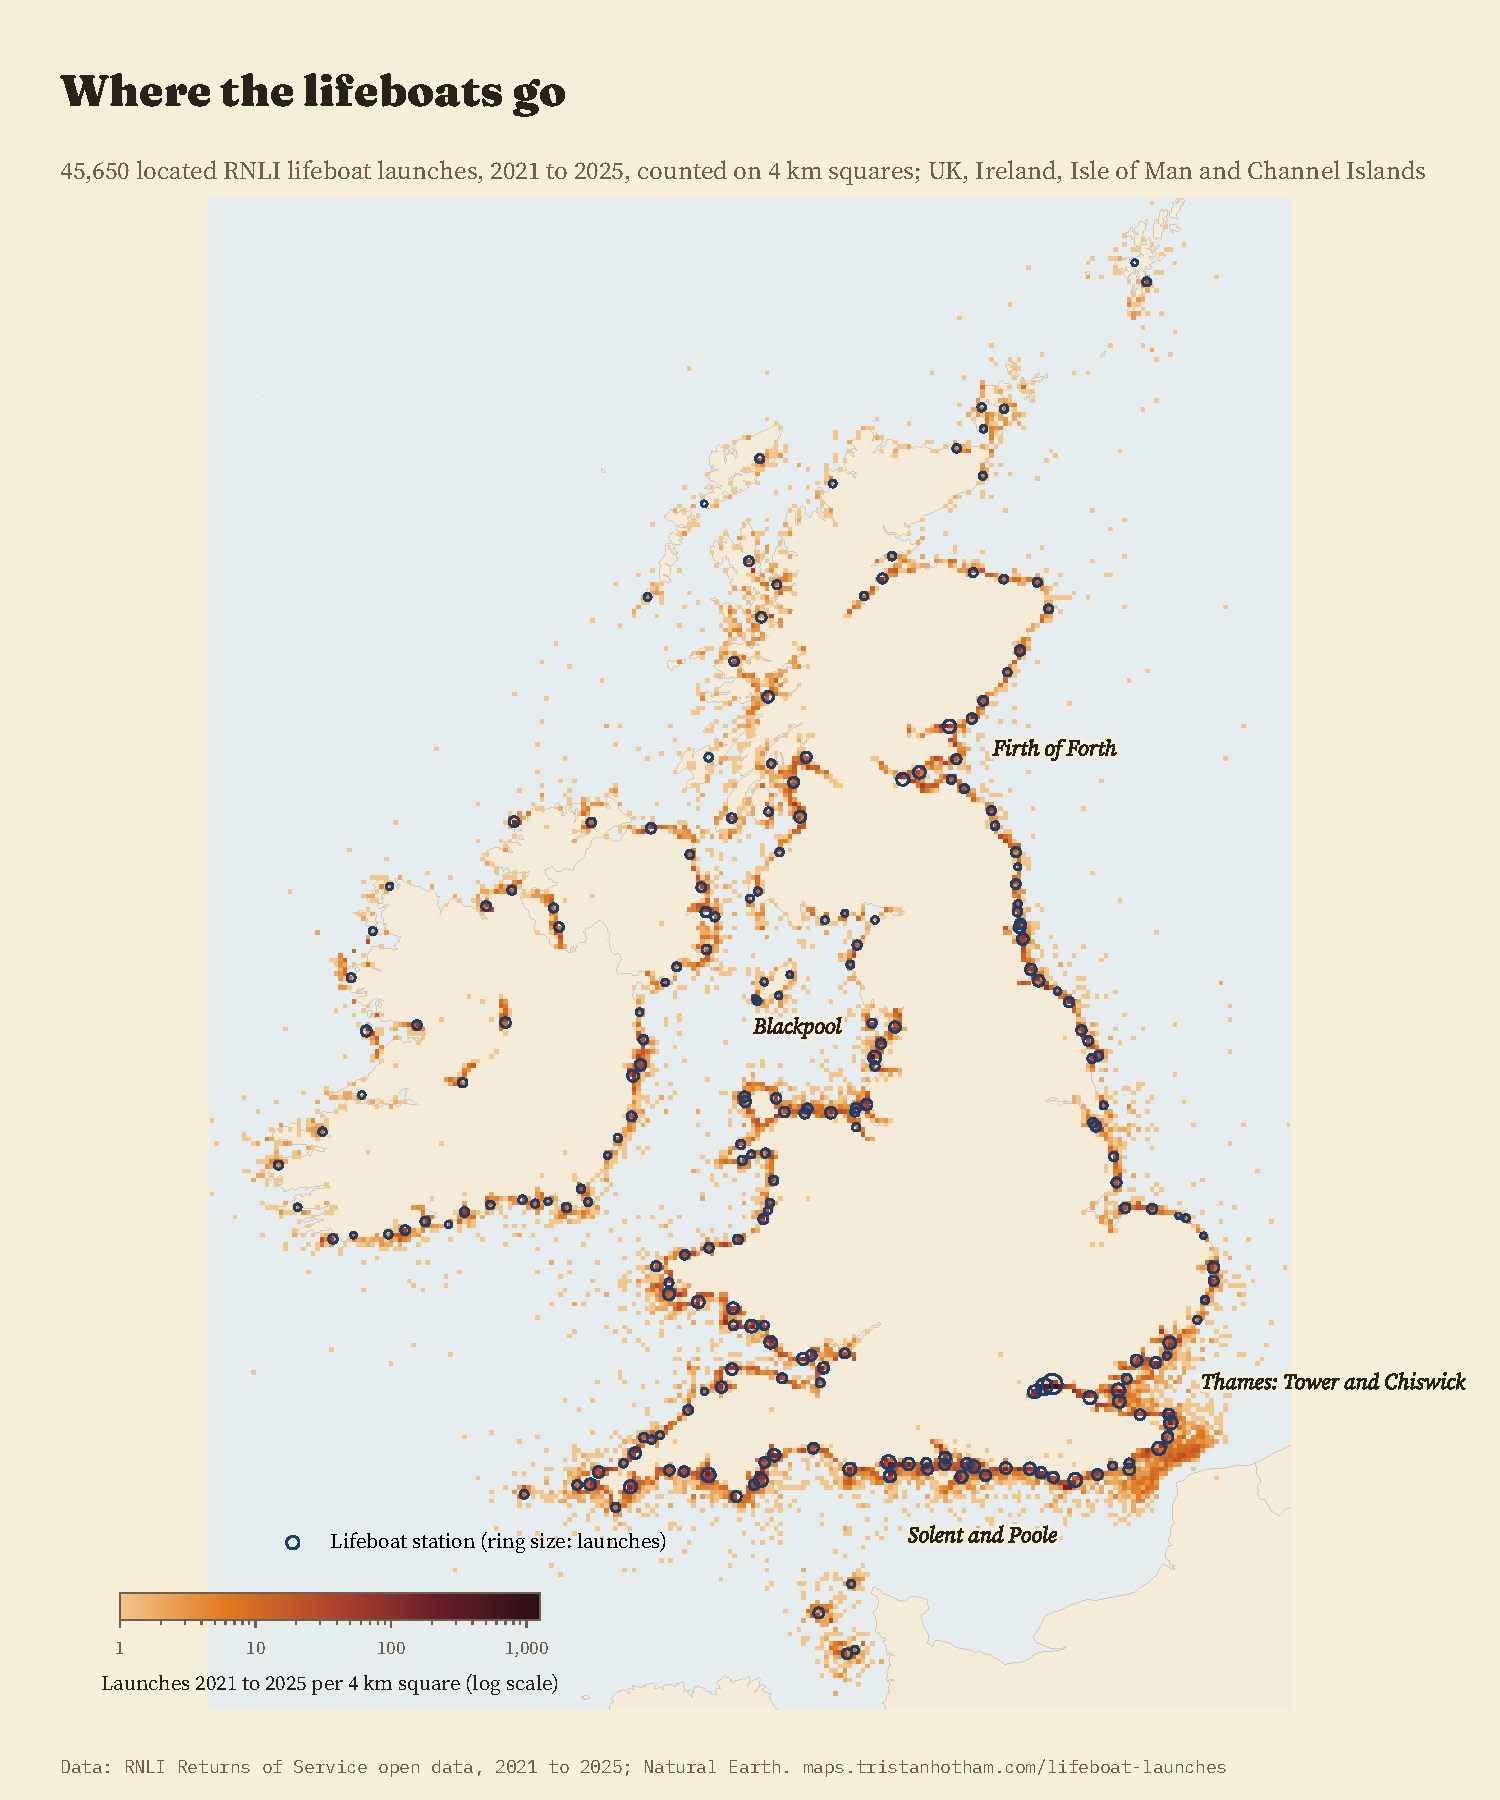
\includegraphics[width=0.78\textwidth]{f_map.pdf}\caption{Located RNLI lifeboat launches, 2021 to 2025, counted on 4 km squares (log colour scale), with stations as rings sized by launches. Coastlines: Natural Earth 1:10m.}\label{fig:map}\end{figure}

\subsection{How far: boat type and casualty (H1, H2)}
Most rescues are close to the station (Figure~\ref{fig:dist}). Half of all located launches went less than 4.5 km (station-cluster bootstrap interval for ALB and ILB launches 3.7 to 5.2 km), 27\% less than 2 km, 77\% less than 10 km, and only 0.7\% more than 50 km. The 90th percentile is 17.2 km.

H1 is supported. The median inshore launch went 3.5 km (95\% interval 3.0 to 4.2) and the median all-weather launch 9.3 km (8.4 to 10.2). 21.8\% of all-weather launches went more than 20 km, against 2.2\% of inshore launches. In the planned model, which compares the two kinds of boat within the same station and month, all-weather launches went 150\% further (95\% CI 119 to 185; $N = 45,082$ launches, 238 stations; Table~\ref{tab:h12}). Among the 68 stations with at least 30 launches of each type, the all-weather boat's median trip was longer at 67, and the median ratio of the two medians was 2.7.

H2 is partly supported. Commercial casualties lay 27\% further from the station than people in the water (CI 16 to 40), holding boat type and station constant. But powered and sail craft were not detectably further than people in the water ($-$4\%, CI $-$11 to 4), and neither were people on the shore ($-$5\%, CI $-$12 to 3). Paddle and board craft were slightly closer ($-$7.4\%, CI $-$14.0 to $-$0.4). The raw medians by group (Figure~\ref{fig:dist}, right) are ordered as expected, with commercial casualties furthest (8.0 km) and people on the shore nearest (3.3 km), but much of that ordering reflects which boats and stations answer which calls: 61\% of commercial launches used an all-weather boat, against 15\% of launches to people on the shore.

\begin{table}[tbp]\centering\small\caption{Planned models for distance (H1, H2): percentage difference in straight-line distance from station to incident, with 95\% confidence intervals clustered by station. OLS of $\log(d+0.1)$.}\label{tab:h12}\begin{tabular}{lll}\toprule & H1 & H2\\\midrule
All-weather lifeboat (vs inshore) & 150 [119, 185] & 145 [115, 179]\\
Commercial (vs people in the water) & & 27 [16, 40]\\
Powered and sail craft (vs people in the water) & & $-$4 [$-$11, 4]\\
Paddle and board craft (vs people in the water) & & $-$7 [$-$14, 0]\\
People on the shore (vs people in the water) & & $-$5 [$-$12, 3]\\
Other or unknown (vs people in the water) & & $-$5 [$-$11, 0]\\
\midrule Station, year and month fixed effects & yes & yes\\
$N$ launches (stations) & 45,082 (238) & 45,082 (238)\\
\bottomrule\end{tabular}\end{table}

\begin{figure}[tbp]\centering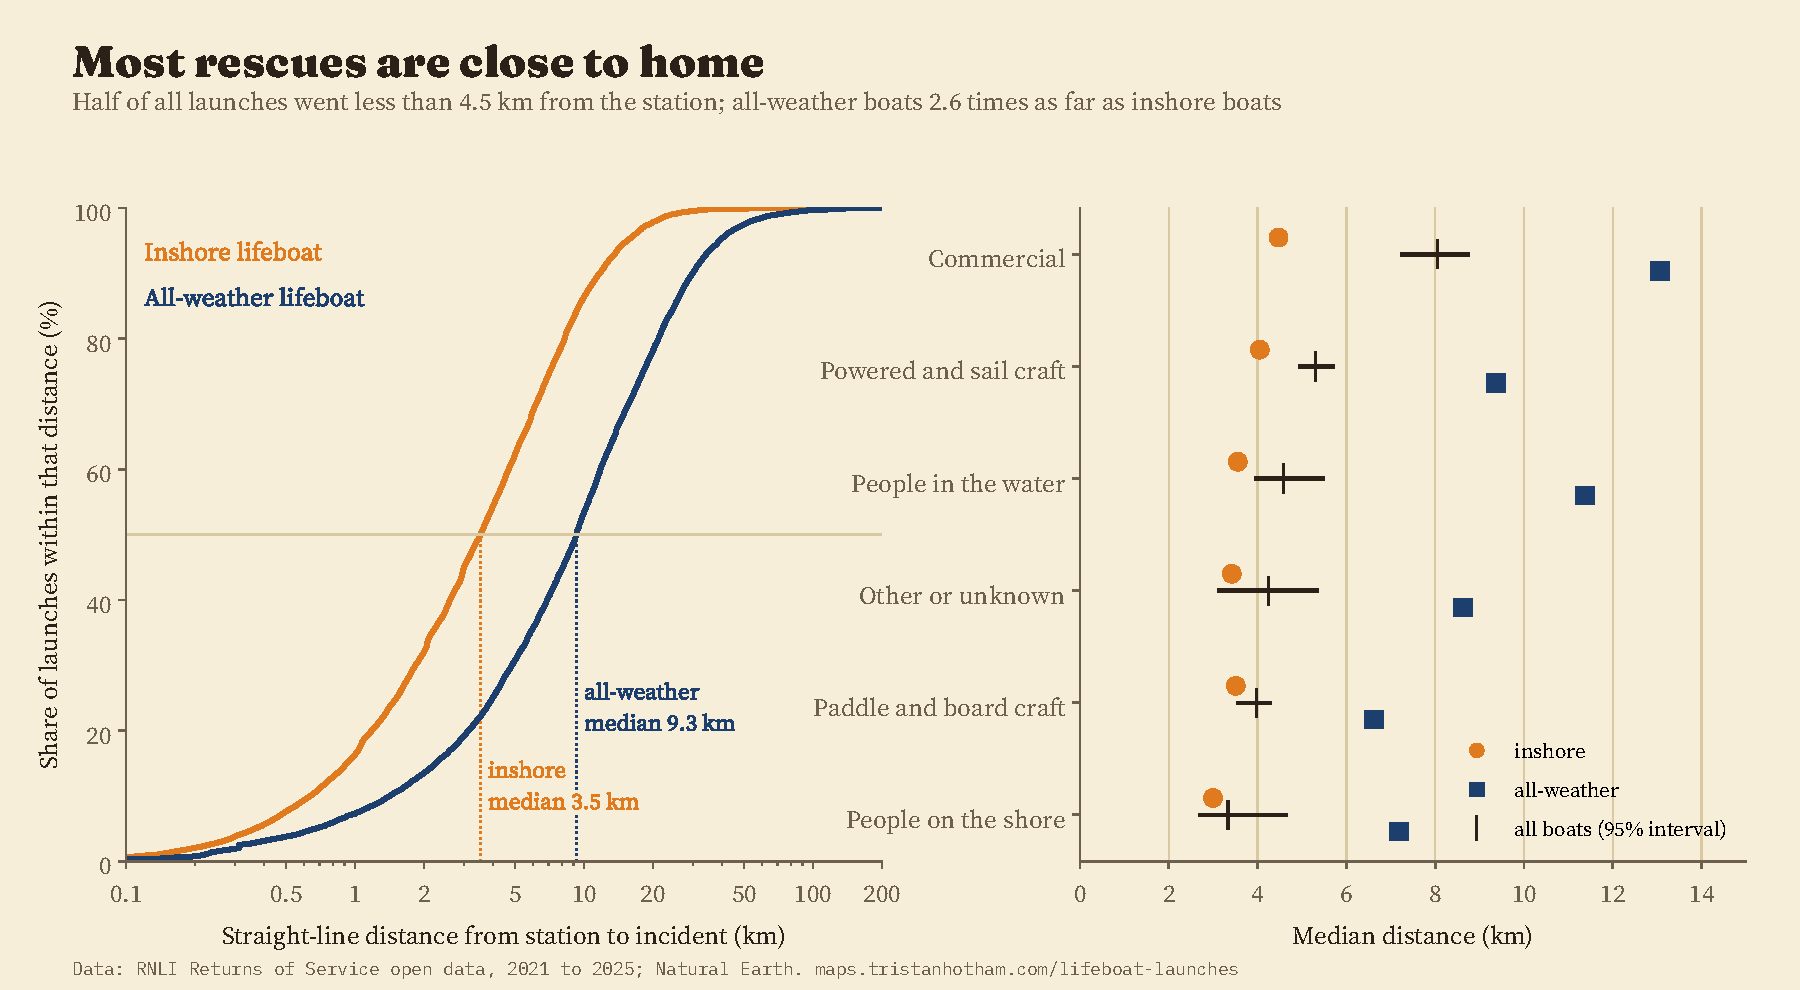
\includegraphics[width=\textwidth]{f_dist.pdf}\caption{Left: cumulative share of located launches by straight-line distance from the station, inshore and all-weather lifeboats. Right: median distance by casualty group (bars: 95\% station-cluster bootstrap intervals for all boats) and by boat type.}\label{fig:dist}\end{figure}

\subsection{When: season, weekend and hour (H3, H3b, H4)}
Launches peak in August, with about 45 a day, against 12 a day in January (3.7 times); June to August hold 42.4\% of all launches and December to February 12.2\%. H3 is supported (Table~\ref{tab:season}, Figure~\ref{fig:season}). The summer-to-winter rate ratio was 10.6 for powered and sail craft (CI 9.2 to 12.1), 6.9 for paddle and board craft and 3.6 for people in the water, against 2.2 for commercial casualties (CI 1.9 to 2.6). The ratio for powered and sail craft is 4.9 times the commercial ratio (CI 3.9 to 6.0). People on the shore and the other or unknown group were no more seasonal than commercial casualties (ratios of ratios 1.11 and 1.10, both with intervals including 1). The three leisure-craft and water contrasts survive a Holm adjustment for the five comparisons.

H3b, the weekend falsification test, is consistent with the leisure reading, though not perfectly. Weekend days brought 2.04 times the weekday rate for paddle and board craft and 1.81 times for powered and sail craft, and the excess over the commercial group's weekend ratio is clear for every group. But commercial casualties were themselves 1.16 times as frequent on weekend days (CI 1.04 to 1.29): not the flat profile I expected. One possible explanation is that the RNLI's commercial category includes charter angling and other commercial activity that peaks at weekends; the data cannot separate these.

Launches follow the day (Figure~\ref{fig:hour}). The busiest hour of launch is 15:00 to 15:59 local time with 3,532 launches, the quietest 5:00 to 5:59 with 493, and 66\% of launches were between 10:00 and 19:59. 22.8\% of located launches were in the dark (Wilson interval 22.4 to 23.2). Paddle and board craft almost never needed a lifeboat after dark (2.4\%, 1.9 to 3.2); powered and sail craft did so in 12.8\% of launches, commercial casualties in 21.8\%, people in the water in 23.9\%, people on the shore in 26.8\% and the other or unknown group in 29.9\%. Against my expectation, all-weather and inshore launches were equally likely to be in the dark (22.6\% and 23.0\%), so the H4 expectation for boat type is not met; the one for commercial casualties is met only relative to leisure craft, not relative to all launches.

\begin{table}[tbp]\centering\scriptsize\caption{Season (H3) and weekend (H3b). Summer (June to August) to winter (December to February) rate ratios from a Poisson model of monthly counts by group with group-by-year fixed effects; their ratio to the commercial group's, with Holm-adjusted p-values for the five contrasts; weekend-day to weekday rate ratios from a Poisson model of daily counts with group-by-month fixed effects, and their ratio to the commercial group's. 95\% intervals from HC1 standard errors.}\label{tab:season}\setlength{\tabcolsep}{3pt}\begin{tabular}{llllll}\toprule Group & Summer/winter & vs commercial & Holm $p$ & Weekend/weekday & vs commercial\\\midrule
Commercial & 2.18 [1.85, 2.56] & (reference) & & 1.16 [1.04, 1.29] & (reference)\\
Powered and sail craft & 10.58 [9.23, 12.12] & 4.85 [3.93, 6.00] & $<$0.001 & 1.81 [1.70, 1.91] & 1.56 [1.38, 1.76]\\
Paddle and board craft & 6.86 [5.41, 8.70] & 3.15 [2.36, 4.20] & $<$0.001 & 2.04 [1.81, 2.29] & 1.76 [1.50, 2.07]\\
People in the water & 3.56 [2.99, 4.24] & 1.64 [1.29, 2.08] & $<$0.001 & 1.43 [1.34, 1.54] & 1.24 [1.09, 1.41]\\
People on the shore & 2.42 [2.12, 2.77] & 1.11 [0.90, 1.37] & 0.630 & 1.39 [1.31, 1.48] & 1.20 [1.06, 1.36]\\
Other or unknown & 2.40 [2.18, 2.63] & 1.10 [0.91, 1.33] & 0.630 & 1.30 [1.24, 1.36] & 1.12 [1.00, 1.26]\\
\bottomrule\end{tabular}\end{table}

\begin{figure}[tbp]\centering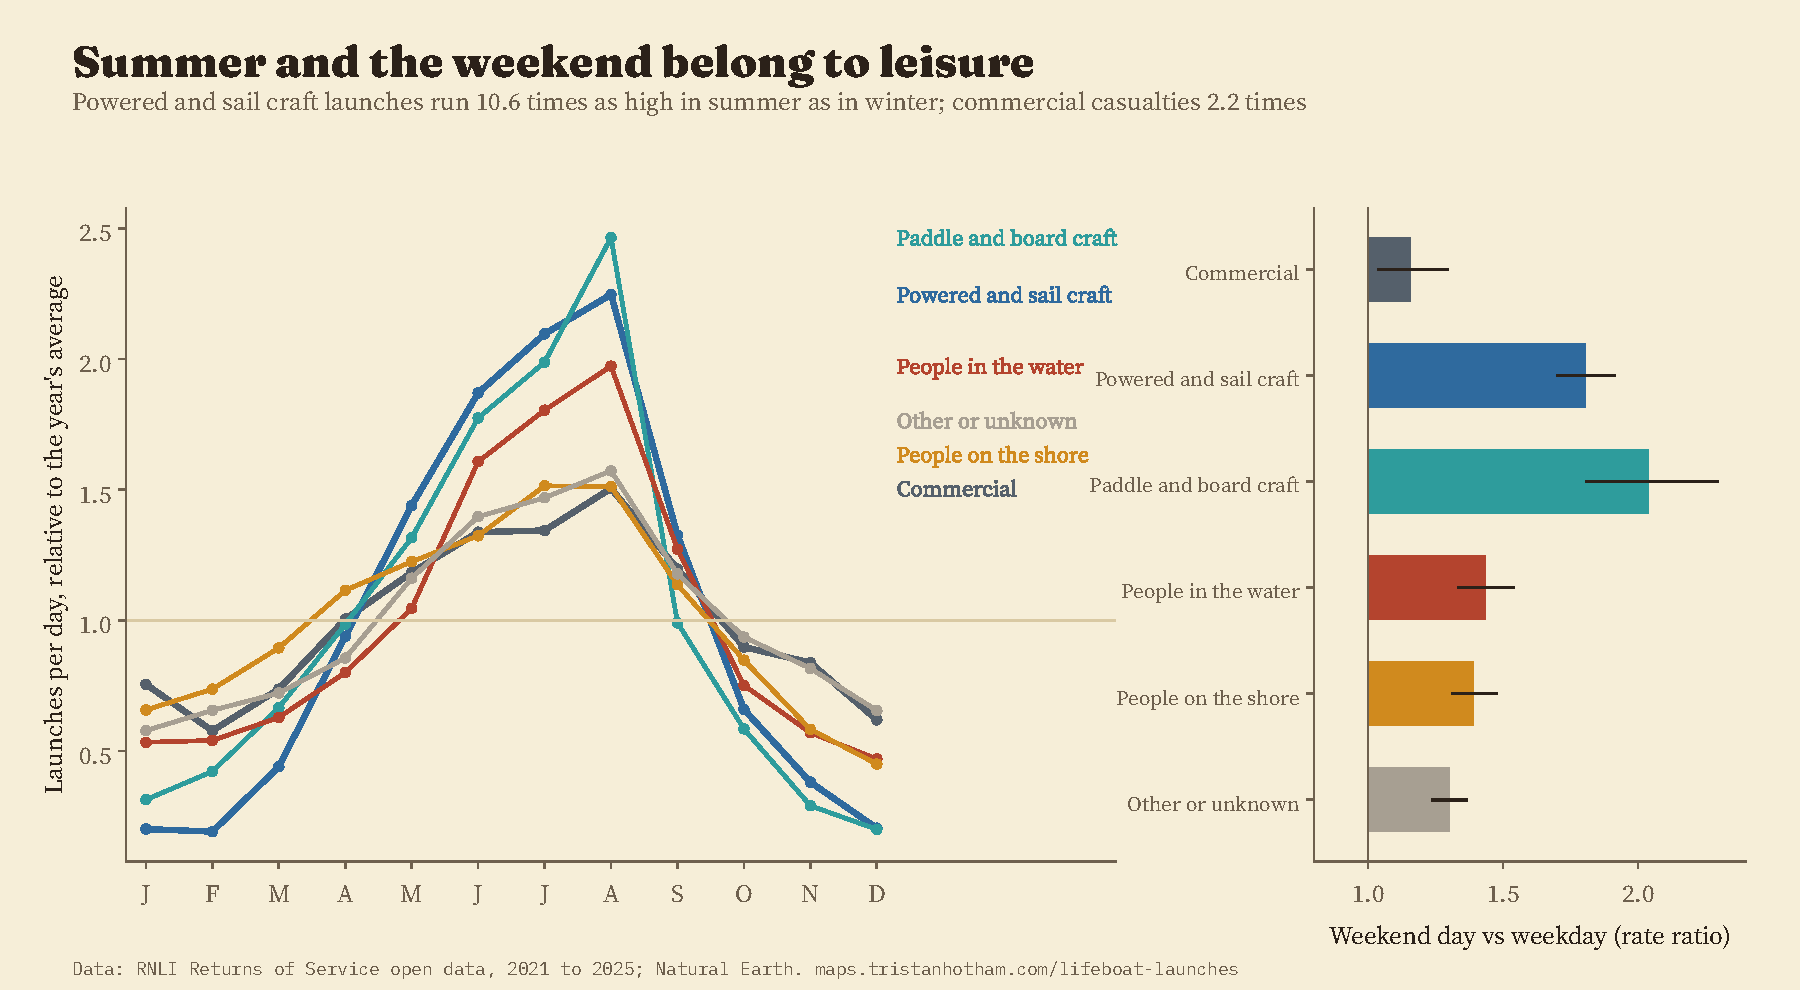
\includegraphics[width=\textwidth]{f_season.pdf}\caption{Left: launches per day in each calendar month, relative to each group's own yearly average, 2021 to 2025. Right: weekend-day to weekday rate ratios by group with 95\% intervals (H3b).}\label{fig:season}\end{figure}

\begin{figure}[tbp]\centering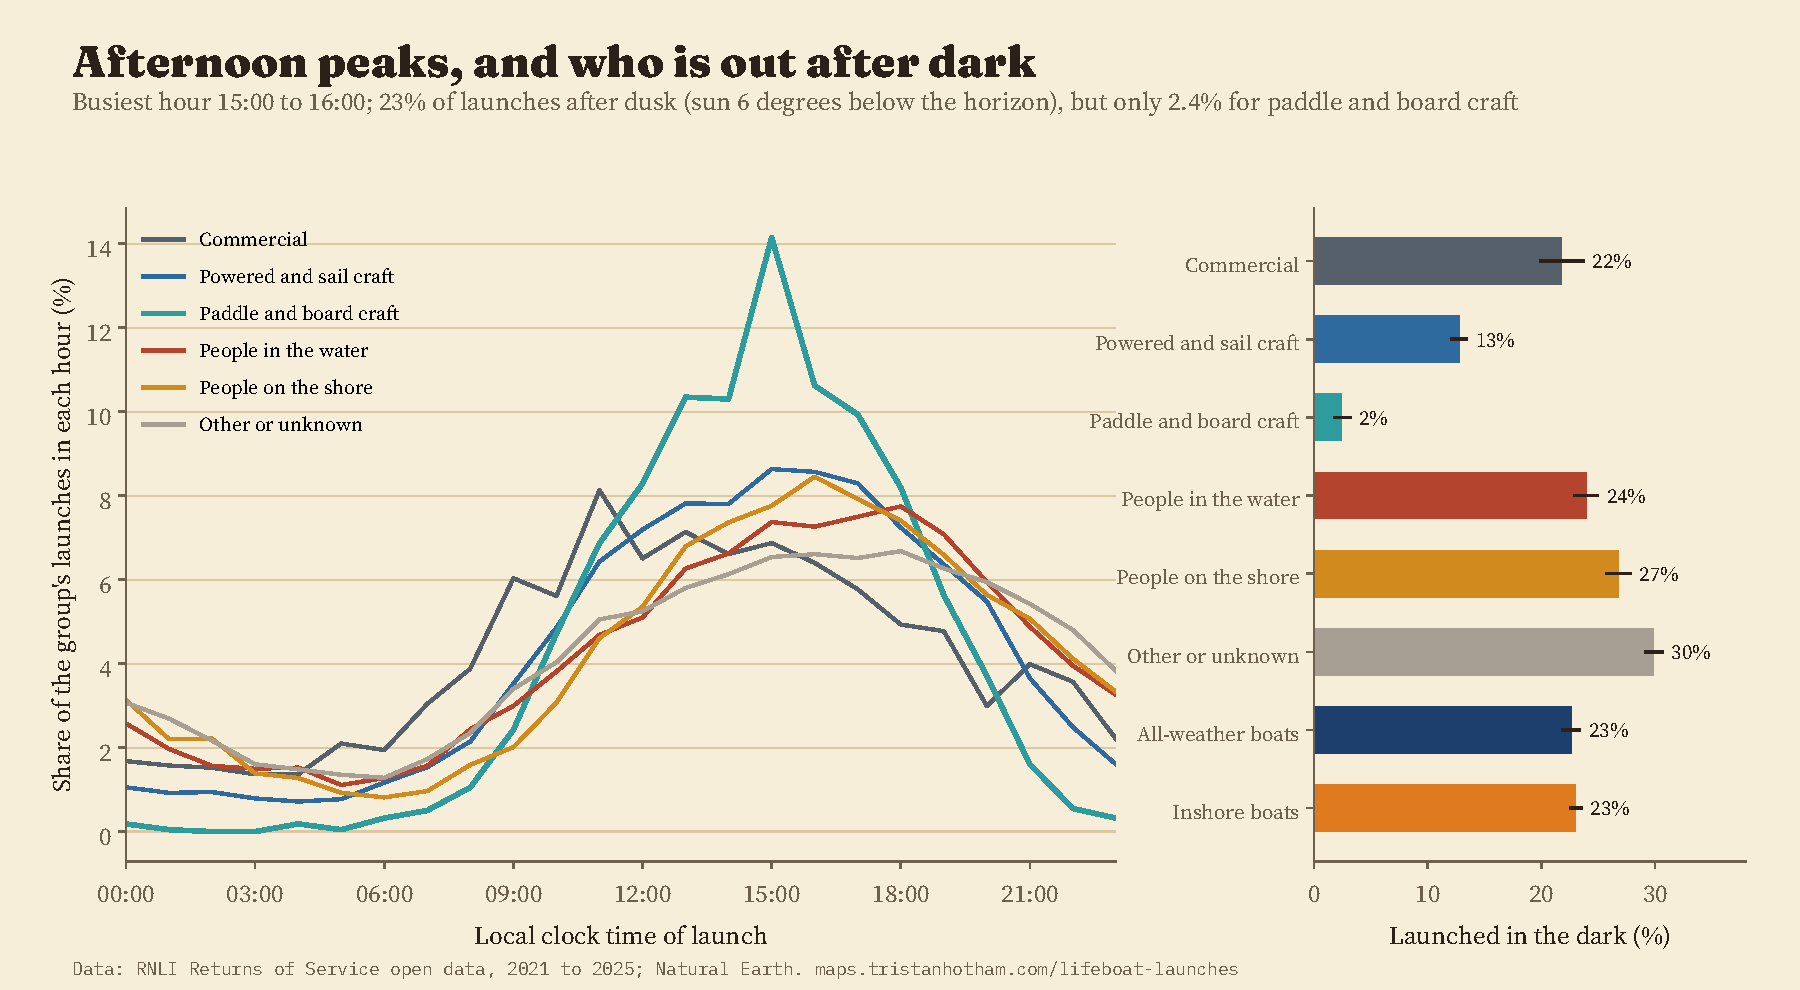
\includegraphics[width=\textwidth]{f_hour.pdf}\caption{Left: share of each group's launches by local clock hour of launch. Right: share of located launches in the dark (sun more than 6 degrees below the horizon at the incident), with Wilson 95\% intervals.}\label{fig:hour}\end{figure}

\subsection{Which stations: workload and coast (H6)}
H6 is supported in the sense planned: launches scale far less than proportionally with coast length (Figure~\ref{fig:coast}, Table~\ref{tab:h6}). The estimated elasticity is 0.098 (CI $-$0.024 to 0.221; $N = 228$ coastal stations): a station with twice as much coast had about 7\% more launches (CI $-$2 to 17\%). The correlation between log coast length and log launches is $-$0.16. Stations with an all-weather boat had 26\% more launches than inshore-only stations in the same region (CI 6 to 49). Per 10 km of coast, the median coastal station made 38 launches in five years; among the 223 stations with at least 10 km of coast, the busiest were Blackpool (437), Ramsgate (358), Torbay (283) and Eastbourne (268), and the quietest were Aith in Shetland and Leverburgh on Harris (0.5 and 0.5), each nearest to more than 400 km of intricate coast at this scale.

The coast-length measure is crude, as Section~\ref{sec:lit} noted, and a better exposure measure would use the numbers of people on the coast and boats at sea, which the open data do not include. The result is best read as a negative finding: coast length alone is a poor guide to where lifeboats are needed.

\begin{table}[tbp]\centering\small\caption{Station workload and coast length (H6): elasticity of five-year launches with respect to the length of coast nearest to each coastal station. Poisson pseudo-maximum likelihood with an all-weather indicator and region fixed effects (main), HC1 95\% intervals; checks below.}\label{tab:h6}\begin{tabular}{lrrl}\toprule Specification & $N$ & Elasticity & 95\% CI\\\midrule
Main model & 228 & 0.098 & [$-$0.024, 0.221]\\
OLS of log launches & 228 & 0.049 & [$-$0.079, 0.177]\\
Coastline at 1:50m & 228 & 0.061 & [$-$0.058, 0.179]\\
Catchment 30 km & 228 & 0.131 & [0.001, 0.260]\\
Without Ireland & 186 & 0.119 & [$-$0.021, 0.258]\\
Without North \& East & 193 & 0.086 & [$-$0.042, 0.214]\\
Without Scotland & 183 & 0.200 & [0.048, 0.352]\\
Without South East & 201 & 0.073 & [$-$0.060, 0.207]\\
Without South West & 195 & 0.051 & [$-$0.071, 0.172]\\
Without Wales \& West & 182 & 0.084 & [$-$0.043, 0.211]\\
\bottomrule\end{tabular}\end{table}

\begin{figure}[tbp]\centering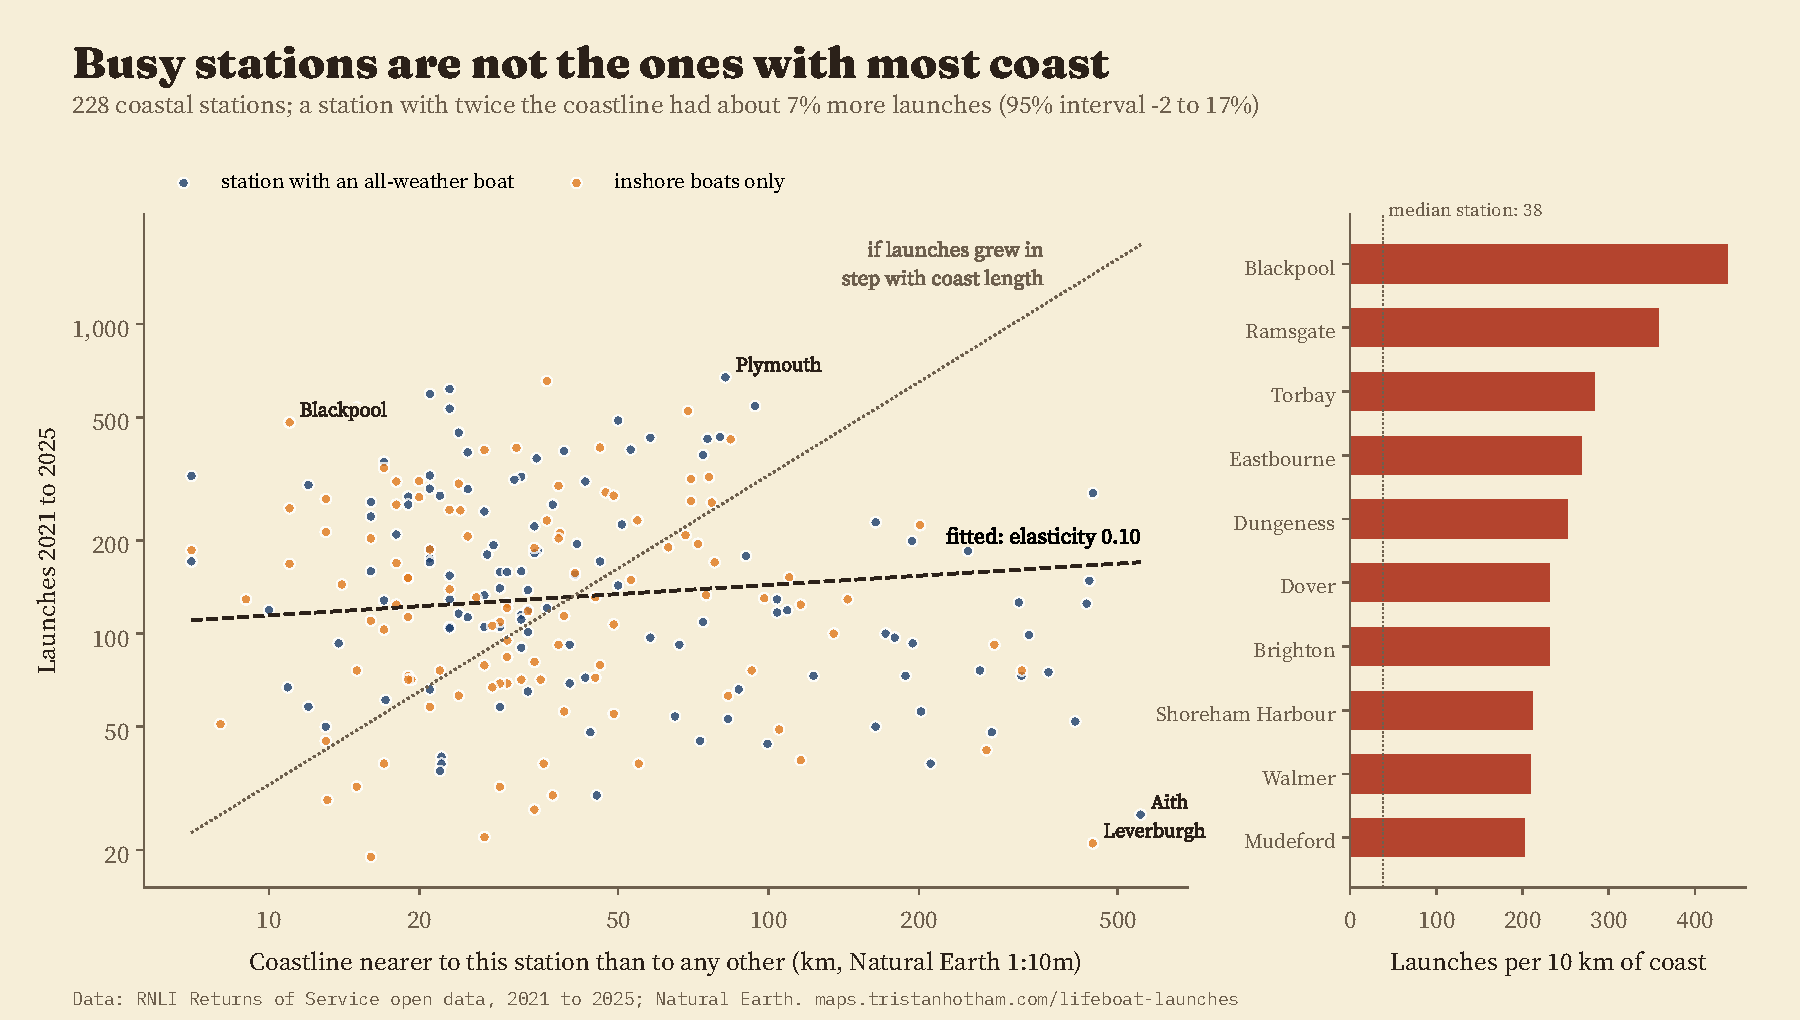
\includegraphics[width=\textwidth]{f_coast.pdf}\caption{Left: launches 2021 to 2025 against the length of Natural Earth 1:10m coastline nearest to each coastal station (log scales), with the fitted Poisson elasticity (dashed) and a line of proportionality (dotted). Right: the ten busiest stations per 10 km of coast among stations with at least 10 km.}\label{fig:coast}\end{figure}

\subsection{Over time (H5)}
Total launches were flat: 8,883 in 2021 and 9,080 in 2025, a trend of 0.3\% a year (CI $-$1.4 to 2.0; Table~\ref{tab:trend}, Figure~\ref{fig:trend}). The planned expectation of a rise in paddle and board launches is not supported: they fell by $-$6.2\% a year (CI $-$8.8 to $-$3.5). Commercial, powered and sail craft and people on the shore also fell, while the other or unknown group rose by 11.5\% a year (CI 10.2 to 12.9).

The rise of the other or unknown group comes mostly from one casualty type, recorded simply as ``Other'', which grew from 727 launches (8.2\%) in 2021 to 1,923 (21.2\%) in 2025, at many stations, including the busiest Thames stations and stations on the coasts of Kent and the Fylde. The reason is not documented in the open data. It may reflect a change in recording practice or a kind of service that the published categories do not name. Either way, with total launches flat, a rising residual category means that the falls in the specific groups cannot be read as real declines in those kinds of emergency: some of them may be launches that are now labelled differently. Exploratory (not in the plan): paddleboard launches alone changed by $-$0.1\% a year (CI $-$6.2 to 6.5).

\begin{table}[tbp]\centering\small\caption{Launches by year and the planned trend estimate (H5): \% change a year from a Poisson model of monthly counts with calendar-month fixed effects and HAC standard errors (12 lags), 95\% intervals.}\label{tab:trend}\setlength{\tabcolsep}{4pt}\begin{tabular}{lrrrrrl}\toprule Group & 2021 & 2022 & 2023 & 2024 & 2025 & \% a year\\\midrule
All launches & 8,883 & 9,316 & 9,205 & 9,189 & 9,080 & 0 [$-$1, 2]\\
Commercial & 442 & 395 & 385 & 321 & 363 & $-$6 [$-$9, $-$2]\\
Powered and sail craft & 2,209 & 2,319 & 2,226 & 1,944 & 1,922 & $-$4 [$-$7, $-$2]\\
Paddle and board craft & 483 & 485 & 430 & 400 & 386 & $-$6 [$-$9, $-$4]\\
People in the water & 1,487 & 1,531 & 1,503 & 1,537 & 1,157 & $-$4 [$-$10, 2]\\
People on the shore & 1,647 & 1,637 & 1,464 & 1,471 & 1,140 & $-$8 [$-$12, $-$3]\\
Other or unknown & 2,615 & 2,949 & 3,197 & 3,516 & 4,112 & 12 [10, 13]\\
\midrule Recorded as ``Other'' (\%) & 8.2 & 9.7 & 12.3 & 16.1 & 21.2 & \\
\bottomrule\end{tabular}\end{table}

\begin{figure}[tbp]\centering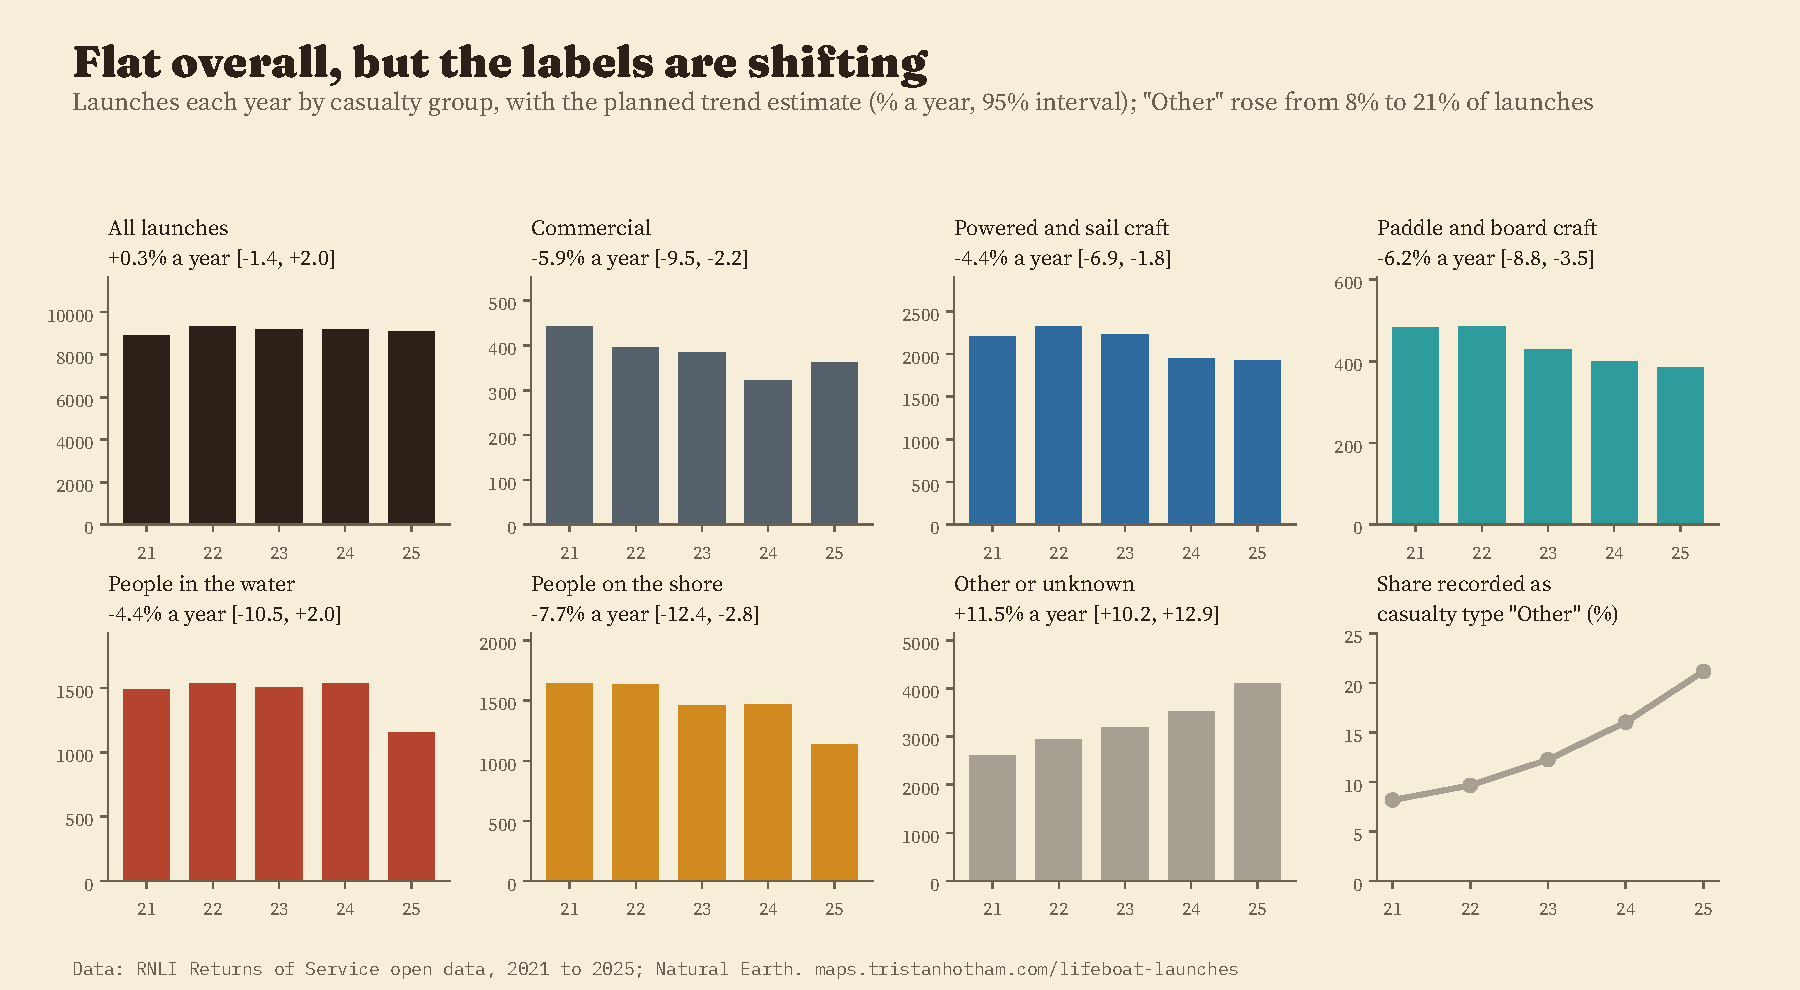
\includegraphics[width=\textwidth]{f_trend.pdf}\caption{Launches each year by casualty group with the planned trend estimates (Poisson, monthly counts, calendar-month fixed effects, HAC errors), and the share of launches recorded with the casualty type ``Other''.}\label{fig:trend}\end{figure}

\section{Robustness}\label{sec:robust}
\textbf{Distance (H1, H2).} The boat-type estimate ranges from 135\% to 162\% across the 14 checks in Table~\ref{tab:robust} and Figure~\ref{fig:robust}, with the lowest lower bound at 103\%. The median regression gives 127\% (CI 121 to 133). In the placebo, permuting boat type within stations 200 times gives coefficients centred on $-$0.03\% with a 95\% range of $-$3.1\% to 3.7\% and a maximum of 6.3\%, against the observed 150\%. The commercial estimate is positive and significant in all 14 checks (range 21\% to 46\%). The powered and sail craft estimate is never significantly positive; it becomes positive and borderline when only launches that arrived on scene, or only launches that were not stood down, are kept (9\% and 6\%), which suggests that some distant calls to leisure craft are cancelled before the boat arrives. The paddle and board estimate is significantly negative in only 7 of the 14 checks, so the finding that these craft are closer than people in the water is not robust.

\textbf{Trend (H5).} The total trend is not significant in any of the 10 checks (range $-$0.8\% to 0.8\% a year). The falls in paddle and board and the rise in other or unknown are significant in all 10; this stability concerns the estimates, not their interpretation, which remains limited by the recording change.

\textbf{Workload (H6).} The elasticity ranges from 0.05 to 0.20 across the 9 checks, is significantly above zero in 2 of them (the 30 km catchment and the model without Scotland), and its upper confidence bound never exceeds 0.35. Measured at 1:50m, where the coast is 9,240 km instead of 15,548 km, the estimate is 0.06.

\begin{figure}[tbp]\centering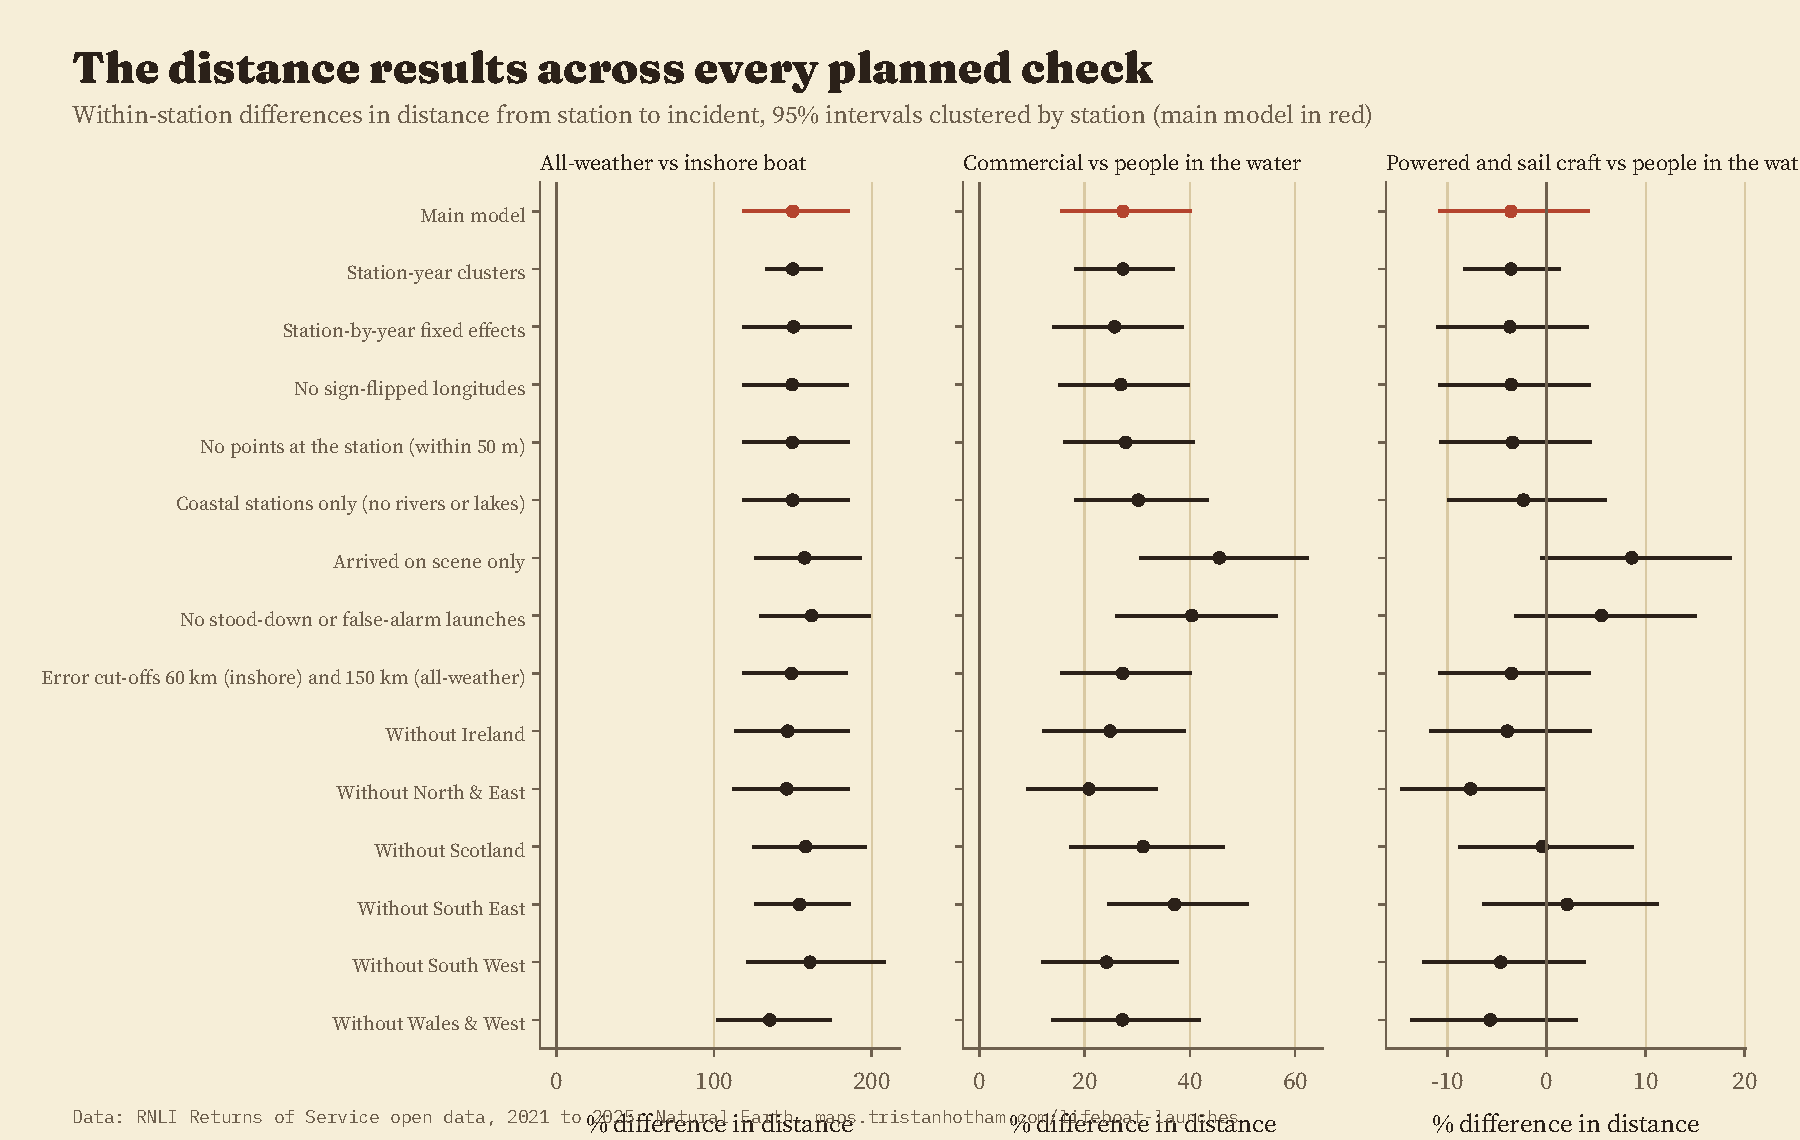
\includegraphics[width=\textwidth]{f_robust.pdf}\caption{Within-station percentage differences in distance from station to incident across all planned checks for H1 and H2, with 95\% intervals clustered by station (main model in red).}\label{fig:robust}\end{figure}

\section{Discussion}\label{sec:disc}
The picture that emerges is of a service whose demand is local and seasonal, with a timing that matches leisure use of the sea. Most launches are to places within a few kilometres of the station; launches to leisure craft multiply in summer and at weekends and are rare after dark; and station workloads bear little relation to the length of the coast around them. The two kinds of lifeboat divide the work as their design suggests: the all-weather boats travel further, and commercial casualties, which they more often attend, lie further out.

Three findings did not match the plan's expectations, and they are informative. Motorboats and yachts were not further from the station than people in the water once station and boat type were held constant. One possible explanation, which these data cannot test, is that most leisure boating happens near harbours and estuaries, close to the stations that serve them, while people in the water can be anywhere along a beach. Commercial casualties were more frequent at weekends too, though less so than leisure ones. And all-weather and inshore boats launched in the dark equally often, which suggests that darkness is a property of the calls rather than of the boats sent to them.

The concentration of launches is striking. Half of all located launches fell in about 6\% of the 2 km squares that saw any launch, and one river station made more than 7\% of all launches. The Thames stations are a reminder that the RNLI's work is not only at sea: on a busy urban river, launches are frequent, short and often in the dark. A national picture that pooled the Thames with the coasts would mislead; this is why the checks drop river and lake stations.

\subsection{Limitations}
\textbf{Launches are not incidents.} A launch is a lifeboat going to sea for a service; several boats sent to one incident produce several rows, and many incidents are handled by coastguard helicopters, lifeguards, other emergency services or the public \citep{odi2021}. The data measure the demand that reached the lifeboats and how it was met, not the risk of the sea.

\textbf{No exposure data.} The data say nothing about how many people or boats were on the water, so seasonal and weekend ratios describe the timing of demand, not the risk per person. Leisure groups may be more seasonal simply because leisure use is.

\textbf{Positions and distances.} Incident positions are recorded by crews and may be approximate; a small number had a lost minus sign or were impossible, and the rules that corrected or excluded them were fixed in advance. Distances are straight lines, which understate the distance travelled around headlands and up estuaries. The 1 km aggregation used for the released data and the map hides the exact positions.

\textbf{Categories change.} The rising share of the casualty type ``Other'' shows that the categories are not stable over the five years. Group-level trends are therefore not reliable, and group-level comparisons pooled over the five years may be affected by the same drift.

\textbf{Coast is a poor exposure measure.} Coast length depends on map scale and ignores population, tourism, harbours and shipping lanes. The coast analysis tests only whether coast alone predicts workload.

\textbf{Five years.} The period includes the end of the pandemic restrictions of early 2021 and four ordinary years; it is too short for a trend analysis to say much about long-run change.

\textbf{Licence.} Because the RNLI's licence restricts redistribution, the release contains aggregates; anyone wishing to reproduce the analysis from the start must obtain the records from the RNLI portal.

\section{Conclusion}\label{sec:conc}
The RNLI's open launch records show a service whose work is mostly close to the station. Half of all launches went less than 4.5 km; all-weather boats went about 2.6 times as far as inshore boats; leisure demand made summer launches to motorboats and yachts about ten times as frequent as winter ones; and station workload bears little relation to coast length. The records are valuable but need care: positions need checking, and the casualty categories have drifted. Further work could link the launches to tides, weather and coastal visitor numbers, compare them with coastguard and lifeguard records, and follow the categories as the RNLI documents its recording practice.

\section*{Data availability statement}
Data and code: Zenodo DOI https://doi.org/10.5281/zenodo.24104520. The interactive page is at \url{https://maps.tristanhotham.com/lifeboat-launches/} and the repository at \url{https://github.com/Tristan-Hotham/lifeboat-launches}. The released data are aggregates (counts by station, month, hour, casualty type and year, and 1 km grid square) under CC BY 4.0; the underlying RNLI launch records are available from the RNLI open data portal under the RNLI's terms and are not redistributed.

\section*{AI statement}
I wrote the text, with drafting and editing assistance from Claude (Anthropic), which also helped prepare the analysis code. I reviewed and checked all text and results.

\begin{thebibliography}{99}
\bibitem[Abadie et al.(2023)]{abadie2023} Abadie, A., Athey, S., Imbens, G. W. and Wooldridge, J. M. (2023) When should you adjust standard errors for clustering? \textit{Quarterly Journal of Economics} 138(1), 1 to 35. doi:10.1093/qje/qjac038.
\bibitem[Boswarva(2018)]{boswarva2018} Boswarva, O. (2018) Blog post on the RNLI open data licence, 4 December 2018. \url{https://owenboswarva.com/blog/post-rnli1.htm}
\bibitem[Cameron and Miller(2015)]{cameron2015} Cameron, A. C. and Miller, D. L. (2015) A practitioner's guide to cluster-robust inference. \textit{Journal of Human Resources} 50(2), 317 to 372.
\bibitem[Efron and Tibshirani(1993)]{efron1993} Efron, B. and Tibshirani, R. J. (1993) \textit{An Introduction to the Bootstrap}. New York: Chapman and Hall.
\bibitem[Holm(1979)]{holm1979} Holm, S. (1979) A simple sequentially rejective multiple test procedure. \textit{Scandinavian Journal of Statistics} 6(2), 65 to 70.
\bibitem[Koenker and Bassett(1978)]{koenker1978} Koenker, R. and Bassett, G. (1978) Regression quantiles. \textit{Econometrica} 46(1), 33 to 50.
\bibitem[Lorenz(1905)]{lorenz1905} Lorenz, M. O. (1905) Methods of measuring the concentration of wealth. \textit{Publications of the American Statistical Association} 9(70), 209 to 219. doi:10.2307/2276207.
\bibitem[MacKinnon and White(1985)]{mackinnon1985} MacKinnon, J. G. and White, H. (1985) Some heteroskedasticity-consistent covariance matrix estimators with improved finite sample properties. \textit{Journal of Econometrics} 29(3), 305 to 325.
\bibitem[Mandelbrot(1967)]{mandelbrot1967} Mandelbrot, B. (1967) How long is the coast of Britain? Statistical self-similarity and fractional dimension. \textit{Science} 156(3775), 636 to 638.
\bibitem[Meeus(1998)]{meeus1998} Meeus, J. (1998) \textit{Astronomical Algorithms}, second edition. Richmond, VA: Willmann-Bell.
\bibitem[Natural Earth(2026)]{naturalearth} Natural Earth (2026) Admin 0 countries (1:10m) and land (1:50m). Public domain. \url{https://www.naturalearthdata.com/}
\bibitem[Open Data Institute(2021)]{odi2021} Open Data Institute (2021) Case study: sharing data to improve the safety of lives at sea. Open Marine Data project, 24 March 2021. \url{https://theodi.org/insights/impact-stories/case-study-sharing-data-to-improve-the-safety-of-lives-at-sea/}
\bibitem[RNLI(2026a)]{rnlidata} RNLI (2026a) Returns of Service; RNLI Lifeboat Station Locations. RNLI open data portal (ArcGIS Hub), retrieved 2026. RNLI open data licence.
\bibitem[RNLI(2026b)]{rnliresearch} RNLI (2026b) Our research. \url{https://rnli.org/about-us/our-research}, retrieved 2026.
\bibitem[Roberts(2018)]{roberts2018} Roberts, W. (2018) Innovate blog: using open data to save lives. RNLI magazine, November 2018. \url{https://rnli.org/magazine/magazine-featured-list/2018/november/innovate-blog-using-open-data-to-save-lives}
\bibitem[Santos Silva and Tenreyro(2006)]{santos2006} Santos Silva, J. M. C. and Tenreyro, S. (2006) The log of gravity. \textit{Review of Economics and Statistics} 88(4), 641 to 658. doi:10.1162/rest.88.4.641.
\bibitem[Seabold and Perktold(2010)]{seabold2010} Seabold, S. and Perktold, J. (2010) statsmodels: econometric and statistical modeling with Python. In \textit{Proceedings of the 9th Python in Science Conference}, 92 to 96.
\bibitem[Wright(2021)]{wright2021} Wright, M. (2021) Part 1: How the RNLI is using geomatics to save lives. \textit{RICS Land Journal}, March 2021 (updated online). \url{https://ww3.rics.org/uk/en/journals/land-journal/how-the-rnli-is-using-geomatics-to-save-lives.html}
\bibitem[Young(2019)]{young2019} Young, A. (2019) Channeling Fisher: randomization tests and the statistical insignificance of seemingly significant experimental results. \textit{Quarterly Journal of Economics} 134(2), 557 to 598.
\bibitem[Akbari et al.(2018)]{akbari2018} Akbari, A., Pelot, R. and Eiselt, H. A. (2018) A modular capacitated multi-objective model for locating maritime search and rescue vessels. \textit{Annals of Operations Research} 267(1), 3 to 28. doi:10.1007/s10479-017-2593-1.
\bibitem[Brander et al.(2013)]{brander2013} Brander, R., Dominey-Howes, D., Champion, C., Del Vecchio, O. and Brighton, B. (2013) Brief communication: a new perspective on the Australian rip current hazard. \textit{Natural Hazards and Earth System Sciences} 13(6), 1687 to 1690. doi:10.5194/nhess-13-1687-2013.
\bibitem[Breivik and Allen(2008)]{breivik2008} Breivik, \O. and Allen, A. A. (2008) An operational search and rescue model for the Norwegian Sea and the North Sea. \textit{Journal of Marine Systems} 69(1 to 2), 99 to 113. doi:10.1016/j.jmarsys.2007.02.010.
\bibitem[Castelle et al.(2016)]{castelle2016} Castelle, B., Scott, T., Brander, R. W. and McCarroll, R. J. (2016) Rip current types, circulation and hazard. \textit{Earth-Science Reviews} 163, 1 to 21. doi:10.1016/j.earscirev.2016.09.008.
\bibitem[Hills et al.(2021)]{hills2021} Hills, S. P., Hobbs, M., Tipton, M. J. and Barwood, M. J. (2021) The water incident database (WAID) 2012 to 2019: a systematic evaluation of the documenting of UK drownings. \textit{BMC Public Health} 21, 1760. doi:10.1186/s12889-021-11827-0.
\bibitem[Hills et al.(2024)]{hills2024} Hills, S. P., Hobbs, M., Brown, P., Tipton, M. and Barwood, M. (2024) Association between air temperature and unintentional drowning risk in the United Kingdom 2012 to 2019: a nationwide case-crossover study. \textit{Preventive Medicine} 179, 107832. doi:10.1016/j.ypmed.2023.107832.
\bibitem[Newey and West(1987)]{newey1987} Newey, W. K. and West, K. D. (1987) A simple, positive semi-definite, heteroskedasticity and autocorrelation consistent covariance matrix. \textit{Econometrica} 55(3), 703 to 708. doi:10.2307/1913610.
\bibitem[Norrington et al.(2008)]{norrington2008} Norrington, L., Quigley, J., Russell, A. and Van der Meer, R. (2008) Modelling the reliability of search and rescue operations with Bayesian Belief Networks. \textit{Reliability Engineering and System Safety} 93(7), 940 to 949. doi:10.1016/j.ress.2007.03.006.
\bibitem[Peden et al.(2016)]{peden2016} Peden, A. E., Franklin, R. C. and Leggat, P. A. (2016) The hidden tragedy of rivers: a decade of unintentional fatal drowning in Australia. \textit{PLoS ONE} 11(8), e0160709. doi:10.1371/journal.pone.0160709.
\bibitem[Pitman et al.(2019)]{pitman2019} Pitman, S. J., Wright, M. and Hocken, R. (2019) An analysis of lifejacket wear, environmental factors, and casualty activity on marine accident fatality rates. \textit{Safety Science} 111, 234 to 242. doi:10.1016/j.ssci.2018.07.016.
\bibitem[Razi and Karatas(2016)]{razi2016} Razi, N. and Karatas, M. (2016) A multi-objective model for locating search and rescue boats. \textit{European Journal of Operational Research} 254(1), 279 to 293. doi:10.1016/j.ejor.2016.03.026.
\bibitem[Scott et al.(2007)]{scott2007} Scott, T., Russell, P., Masselink, G., Wooler, A. and Short, A. (2007) Beach rescue statistics and their relation to nearshore morphology and hazards: a case study for southwest England. \textit{Journal of Coastal Research} Special Issue 50, 1 to 6.
\bibitem[Szpilman et al.(2012)]{szpilman2012} Szpilman, D., Bierens, J. J. L. M., Handley, A. J. and Orlowski, J. P. (2012) Drowning. \textit{New England Journal of Medicine} 366(22), 2102 to 2110. doi:10.1056/NEJMra1013317.
\bibitem[Weisburd(2015)]{weisburd2015} Weisburd, D. (2015) The law of crime concentration and the criminology of place. \textit{Criminology} 53(2), 133 to 157. doi:10.1111/1745-9125.12070.
\bibitem[Willcox-Pidgeon et al.(2019)]{willcoxpidgeon2019} Willcox-Pidgeon, S., Peden, A. E., Franklin, R. C. and Scarr, J. (2019) Boating-related drowning in Australia: epidemiology, risk factors and the regulatory environment. \textit{Journal of Safety Research} 70, 117 to 125. doi:10.1016/j.jsr.2019.06.005.
\bibitem[Wilson(1927)]{wilson1927} Wilson, E. B. (1927) Probable inference, the law of succession, and statistical inference. \textit{Journal of the American Statistical Association} 22(158), 209 to 212. doi:10.2307/2276774.
\bibitem[Woodward et al.(2013)]{woodward2013} Woodward, E., Beaumont, E., Russell, P., Wooler, A. and Macleod, R. (2013) Analysis of rip current incidents and victim demographics in the UK. \textit{Journal of Coastal Research} Special Issue 65, 850 to 855. doi:10.2112/SI65-144.1.
\end{thebibliography}

\appendix
\section{Additional tables}
\begin{table}[tbp]\centering\scriptsize\caption{Robustness of the distance models (H1, H2): percentage differences with 95\% intervals for all-weather vs inshore boats and for commercial, powered and sail craft, paddle and board craft and people on the shore vs people in the water.}\label{tab:robust}\setlength{\tabcolsep}{2pt}\resizebox{\textwidth}{!}{\begin{tabular}{p{5.4cm}rlllll}\toprule Check & $N$ & All-weather & Commercial & Powered/sail & Paddle/board & Shore\\\midrule
Main model & 45,082 & 150 [119, 185] & 27 [16, 40] & $-$4 [$-$11, 4] & $-$7 [$-$14, 0] & $-$5 [$-$12, 3]\\
\midrule
\multicolumn{7}{l}{\textit{Inference}}\\
\quad Station-year clusters & 45,082 & 150 [133, 168] & 27 [18, 37] & $-$4 [$-$8, 1] & $-$7 [$-$12, $-$2] & $-$5 [$-$9, 0]\\
\multicolumn{7}{l}{\textit{Specification}}\\
\quad Station-by-year fixed effects & 45,082 & 150 [119, 187] & 26 [14, 38] & $-$4 [$-$11, 4] & $-$7 [$-$13, 1] & $-$5 [$-$12, 4]\\
\multicolumn{7}{l}{\textit{Measurement}}\\
\quad No sign-flipped longitudes & 44,947 & 150 [119, 184] & 27 [15, 40] & $-$4 [$-$11, 4] & $-$7 [$-$14, 0] & $-$5 [$-$12, 3]\\
\quad No points at the station (within 50 m) & 45,027 & 150 [119, 185] & 28 [16, 41] & $-$3 [$-$11, 4] & $-$7 [$-$14, 0] & $-$5 [$-$12, 3]\\
\quad Coastal stations only (no rivers or lakes) & 38,961 & 150 [119, 185] & 30 [18, 43] & $-$2 [$-$10, 6] & $-$6 [$-$13, 1] & $-$3 [$-$11, 6]\\
\multicolumn{7}{l}{\textit{Sample}}\\
\quad Arrived on scene only & 40,381 & 157 [127, 192] & 46 [31, 62] & 9 [0, 18] & 4 [$-$4, 13] & 2 [$-$7, 13]\\
\quad No stood-down or false-alarm launches & 38,462 & 162 [130, 198] & 40 [26, 56] & 6 [$-$3, 15] & 1 [$-$7, 10] & 2 [$-$7, 12]\\
\multicolumn{7}{l}{\textit{Measurement}}\\
\quad Error cut-offs 60 km (inshore) and 150 km (all-weather) & 45,057 & 149 [119, 184] & 27 [16, 40] & $-$4 [$-$11, 4] & $-$7 [$-$14, 0] & $-$4 [$-$12, 3]\\
\multicolumn{7}{l}{\textit{Leave one region out}}\\
\quad Without Ireland & 40,150 & 147 [114, 185] & 25 [12, 39] & $-$4 [$-$12, 4] & $-$9 [$-$16, $-$2] & $-$4 [$-$12, 5]\\
\quad Without North \& East & 39,559 & 146 [113, 185] & 21 [9, 34] & $-$8 [$-$15, 0] & $-$10 [$-$17, $-$2] & $-$7 [$-$14, 1]\\
\quad Without Scotland & 39,173 & 158 [125, 196] & 31 [17, 46] & 0 [$-$9, 9] & $-$7 [$-$15, 0] & $-$3 [$-$11, 6]\\
\quad Without South East & 31,045 & 154 [127, 185] & 37 [25, 51] & 2 [$-$6, 11] & $-$3 [$-$10, 5] & $-$2 [$-$11, 8]\\
\quad Without South West & 37,813 & 161 [121, 208] & 24 [12, 38] & $-$5 [$-$12, 4] & $-$8 [$-$15, 0] & $-$5 [$-$13, 4]\\
\quad Without Wales \& West & 37,670 & 135 [103, 173] & 27 [14, 42] & $-$6 [$-$14, 3] & $-$6 [$-$13, 2] & $-$6 [$-$14, 2]\\
\multicolumn{7}{l}{\textit{Median regression}}\\
\quad Quantile 0.5, station indicators & 45,082 & 127 [121, 133] & 33 [27, 39] & $-$4 [$-$7, $-$1] & $-$10 [$-$14, $-$6] & $-$2 [$-$5, 1]\\
\bottomrule\end{tabular}}\end{table}

\begin{table}[tbp]\centering\small\caption{The fifteen busiest stations, 2021 to 2025: type (ALB: has an all-weather boat), RNLI region, launches, median distance (km) and launches per 10 km of nearest coast (blank for river stations).}\label{tab:stations}\begin{tabular}{lllrrr}\toprule Station & Type & Region & Launches & Median km & Per 10 km\\\midrule
Tower & ILB & South East & 3,077 & 2.1 & \\
Chiswick & ILB & South East & 1,388 & 2.8 & \\
Plymouth & ALB & South West & 673 & 3.6 & 82\\
Poole & ILB & South East & 654 & 4.9 & 182\\
Eastbourne & ALB & South East & 617 & 8.5 & 268\\
Torbay & ALB & South West & 595 & 5.5 & 283\\
Broughty Ferry & ALB & Scotland & 543 & 5.2 & 58\\
Ramsgate & ALB & South East & 537 & 5.5 & 358\\
Dover & ALB & South East & 533 & 16.0 & 232\\
Southend-on-Sea & ILB & South East & 523 & 3.3 & 76\\
Falmouth & ALB & South West & 488 & 4.0 & 98\\
Gravesend & ILB & South East & 484 & 12.5 & \\
Blackpool & ILB & Wales \& West & 481 & 1.1 & 437\\
Teddington & ILB & South East & 453 & 2.5 & \\
The Mumbles & ALB & Wales \& West & 446 & 3.0 & 186\\
\bottomrule\end{tabular}\end{table}

\begin{table}[tbp]\centering\scriptsize\caption{Casualty groups and the RNLI casualty types they contain, with launches 2021 to 2025 (each type listed under the group most of its launches fall in; commercial is the RNLI's commercial category, which overrides the type).}\label{tab:types}\begin{tabular}{lp{12.2cm}}\toprule Group & Casualty types (launches)\\\midrule
Commercial & Commercial fishing (1,437), Commercial activity (369)\\
Powered and sail craft & Motorboat (5,407), Sailing vessel (3,836), Angler from boat (427), Jet ski (392), Inflatable (335), Sailing dinghy (228), Rowing boat (124), Diving vessel (72), Waterskier (11)\\
Paddle and board craft & Kayak/canoe (857), Paddleboard (760), Kitesurf (233), Windsurf (178), Surfboard (80), Bodyboard (75), Skimboard (1)\\
People in the water & Person in water (5,964), Swimmer (691), Multiple persons on the water (390), Scuba diver (106), Tombstoner (67)\\
People on the shore & Person ashore (4,408), Walker/runner (1,686), Waterside activity (382), Animal (dog) (308), Animal (other) (209), Climber (152), Angler from shore (143), Motor vehicle (40), Coasteerer (31)\\
Other or unknown & Other (6,155), Person in distress (3,149), Person on craft (1,839), False alarm (1,657), Unknown craft (1,623), Unknown person (1,597), Mass rescue (90), Unknown (72), Aircraft (46), Distress signals (28), Object in the sea (18)\\
\bottomrule\end{tabular}\end{table}

\section{Data construction}\label{app:data}
\textbf{Pipeline.} \texttt{01\_data.py} reads the launch records and station list, applies the cleaning rules, computes distances, darkness and the coast allocation; \texttt{02\_models.py} runs the planned models and checks; \texttt{03\_results.py} writes every number quoted in this paper to \texttt{results.json}, with assertions for claims made in words, and writes the aggregate data files. Every number in this paper is filled from that file.

\textbf{Rules.} C1 station matching by folded name, Chiswick placed at the median of its launches, training launches dropped; C2 longitude sign flipped when the flipped point is within 60 km of the station and the original more than twice as far; C3 location errors beyond 100 km (inshore, hovercraft, water craft) or 250 km (all-weather); C4 points within 50 m of the station flagged; C5 river and lake stations (more than 3 km from the 1:10m coastline, or on the Thames); C6 casualty groups (Table~\ref{tab:types}); C7 boat type from the RoS type field, with 4 launches of unknown type excluded from boat comparisons; C8 great-circle distance; C9 coast allocation to the nearest coastal station within 60 km on 1 km pieces in EPSG:3035; C10 darkness when the solar altitude is below $-6$ degrees.

\textbf{Released data.} Station table (attributes, coast length, counts by year, boat and group, median distance, share in the dark); monthly counts by group; hourly counts by group and boat; launches by casualty type and year; launch counts on a 1 km grid (cell centre, totals by year, boat and group); all model coefficients.

\end{document}
